\documentclass[a4paper,11pt,oneside]{book}
\usepackage[final]{graphicx}
\usepackage{subcaption}
\usepackage[utf8]{inputenc}
\usepackage{graphicx}
\usepackage[english]{babel}
\usepackage[backend=biber,citestyle=numeric-comp,sorting=none]{biblatex}
\usepackage{array}
\usepackage{float}
\usepackage{tfrupee}
\usepackage{siunitx}
\usepackage[section]{placeins}
\usepackage{verbatim}
\usepackage{listings}
\usepackage{hyperref}
\usepackage[hashEnumerators,smartEllipses]{markdown}


\addbibresource{references.bib}

\graphicspath{ {./figures/} }

\newcommand{\ProjectTitle}{DFPL Project001}

\pagenumbering{arabic}

\begin{document}

\begin{titlepage}
\begin{center}
\fontsize{28pt}{30pt}\selectfont
\textbf{DOCUMENTATION}\\[0.5cm]
\fontsize{20pt}{30pt}\selectfont
of\\[0.5cm]
\fontsize{32pt}{32pt}\selectfont
\textbf{\ProjectTitle}\\[14cm]
\fontsize{16pt}{18pt}\selectfont
\textbf{December 2019}
\end{center}
\end{titlepage}

\newpage
\tableofcontents

\newpage
\thispagestyle{empty}

\addcontentsline{toc}{chapter}{List of Figures}
\listoffigures

\addcontentsline{toc}{chapter}{List of Tables}
\listoftables

\mainmatter
\newpage

\chapter{Prerequisite Concepts}
\section{Internet of Things}
Internet of Things (IoT) \cite{BandaCM15} is an ecosystem of devices that are connected to the internet. The ‘thing’ can be anything from a heart monitor, an automobile, temperature sensor to a refrigerator. It includes any object that can transmit or receive data either directly or indirectly to the internet without manual assistance. The advent of wireless technology has lead to a rapid decrease in costs of such a system and increased the viability of a large deployment of IoT devices exponentially.

The devices are managed using an IoT platform which is a multi-layer technology that enables straightforward provisioning and management of connected devices. This has lead to IoT being widely used in connecting devices and collecting data information. The system is used to register their sensors, manage streams of data and handle configuration updates. Using a cloud-based service for the same greatly speeds up the development of applications and takes care of scalability and cross-device compatibility as well \cite{ref1.4}.

This connects your diverse hardware using a range of enterprise-grade connectivity options to huge data processing solutions, opening up a plethora of applications ranging from data collection to drone delivery networks to precision farming \cite{iotPAhighLevel}.

\section{Wireless Sensor Network}

A Wireless sensor network (WSN) refers to a group of spatially dispersed connected sensors that can be used for monitoring and recording the environmental conditions and creating a network to route that data to a central location. WSNs in precision farming increase efficiency and profitability by reducing networking costs and deployment complexity \cite{ref2.2}. This gives real-time access to environmental information remotely which can be used for storage, data analytics, and make resource decisions. This contrasts with the traditional agricultural methods in which decisions were taken based on tradition and habit.

%include reference to this
\begin{figure}[!h]
  \centering
  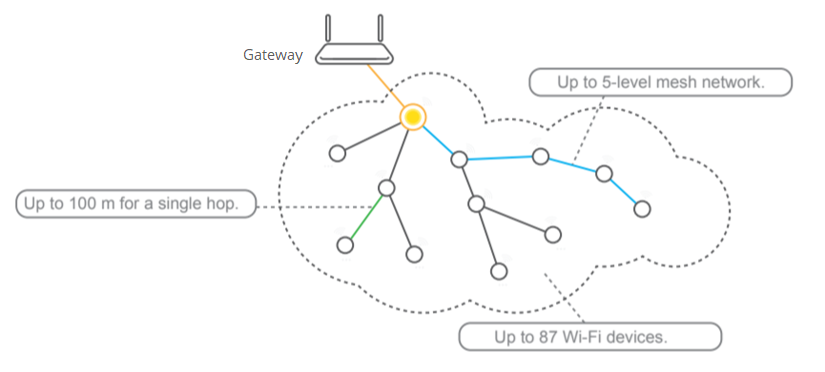
\includegraphics[width=\textwidth]{mesh.png}
  \caption{ESP8266 Mesh Network}
  \label{fig:mesh}
\end{figure}

WSNs make a large scale deployment of sensors economically viable for the farming domain \cite{pfWSN}. It supports many operations such as irrigation, fertilizer use, soil monitoring and intruder detection \cite{main3}. Its integration has resulted in a plethora of applications such as remote healthcare, water control, precision agriculture, smart cities, and wildlife monitoring \cite{main2}.

\section{Gateway}
An IoT gateway is a device/software that serves as the bridge between the WSN and the cloud side. It is responsible for device management, data processing, and routing \cite{usingGateways}.

\noindent
In a cloud-based network architecture, these gateways act as edge nodes, reducing the amount of processing power required on the cloud end. As seen in Figure~\ref{fig:gateway}, this reduces both the cost and the complexity of the network. 

\begin{figure}[h]
  \centering
  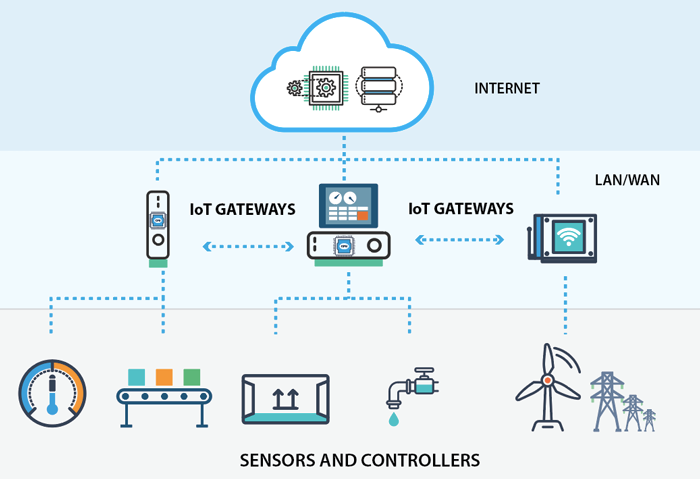
\includegraphics[width=0.9\textwidth]{gateway.png}
  \caption{Role of an IoT Gateway \cite{whatGateway}}
  \label{fig:gateway}
\end{figure}

\noindent
It performs several tasks on their behalf, such as: \cite{usingGateways}
\begin{itemize}
  \item Communicating with IoT Platform;
  \item Connecting to the internet when the device can't directly connect itself, such as a ZigBee or Bluetooth device;
  \item Providing secure authentication when the device can't send its credentials, or when you want to add a layer of security by using the credentials of both the device and the gateway;
  \item Publishing telemetry events, device management, getting configuration data, or setting device state;
  \item Storing and processing data, logs and telemetry; and
  \item Translating between different protocols.
\end{itemize}




\newpage
\chapter{Solution Architecture}
\section{Requirements and Design Consideration}

\noindent
The requirements for this project are clear and fixed. The functional requirements are as follows:
\begin{enumerate}
  \item The platform should scale easily with the number of devices and sensing parameters;
  \item WSN should be inexpensive and easy to deploy;
  \item The platform should have archival cloud storage with data analytics capability;
  \item The cloud service must be reliable and always on;
  \item Devices must be authenticated before sending telemetry data;
  \item Devices should be managed and reconfigured via over-the-air (OTA) updates;
  \item Data should be accessible in real-time by the user via MQTT; and
  \item The telemetry parameters required for each sensing node are given in Table~\ref{table:telemetryParameters}.
\end{enumerate}

\renewcommand{\floatpagefraction}{0.9}
\renewcommand{\arraystretch}{1.1}
\begin{table}[ht]
\centering
\begin{tabular}{ p{5.2cm} p{6.2cm}}
  \hline
  \textbf{Service Type} & \textbf{Telemetry Parameters}\\
  \hline
  Publish & Soil Temperature\\
  & Soil Moisture\\
  & Timestamp\\
  & NodeID\\
  & FarmID\\
  \hline
  Subscribe & Configuration State\\
  & Commands\\
  \hline
\end{tabular}
\caption{Device Telemetry Parameters} 
\label{table:telemetryParameters}
\end{table} 

\noindent
Based on the functional requirement, the proposed Software Design Considerations are given in Table~\ref{table:designConsideration}.

\renewcommand{\arraystretch}{1.2}
\begin{table}[ht]
\centering
\begin{tabular}{ p{0.4cm} p{5cm} p{6cm}}
  \hline
  & \textbf{Requirement} & \textbf{Design Consideration}\\
  \hline
  1 & Scalable with the number of devices and sensing parameters & An easily scalable WSN to be used.\\
  2 & WSN should be inexpensive and easy to deploy & WSN shouldn't be based on proprietary software/hardware; preferably consumer hardware\\
  3 & Cloud Platform must have archival cloud storage with data analytics capability & Utilizing Google BigQuery for its high throughput and big data analytics capability\\
  4 & Cloud service must be reliable and always on & Google Cloud Platform is reliable and has high availability\\
  5 & Devices must be authenticated before sending telemetry data & Sensing nodes will be authenticated using an intermediary device keeping the cost down\\
  6 & Devices should be managed and reconfigured via over-the-air (OTA) updates & GCP IoT Core provides device management and configuration over the air\\
  7 & Data should be accessible in real-time by the user via MQTT & Real-time data will be made available through an MQTT broker hosted by Google Cloud Pub/Sub\\
  \hline
\end{tabular}
\caption{Functional Requirements and Design Considerations} 
\label{table:designConsideration}
\end{table} 

\newpage
\section{Network Architecture}

The proposed network architecture (depicted in Figure~\ref{fig:layers}) is composed of 3 layers: sensor, gateway, and cloud back-end. In this section, we will discuss these three layers and their implementation.

\begin{figure}[!h]
  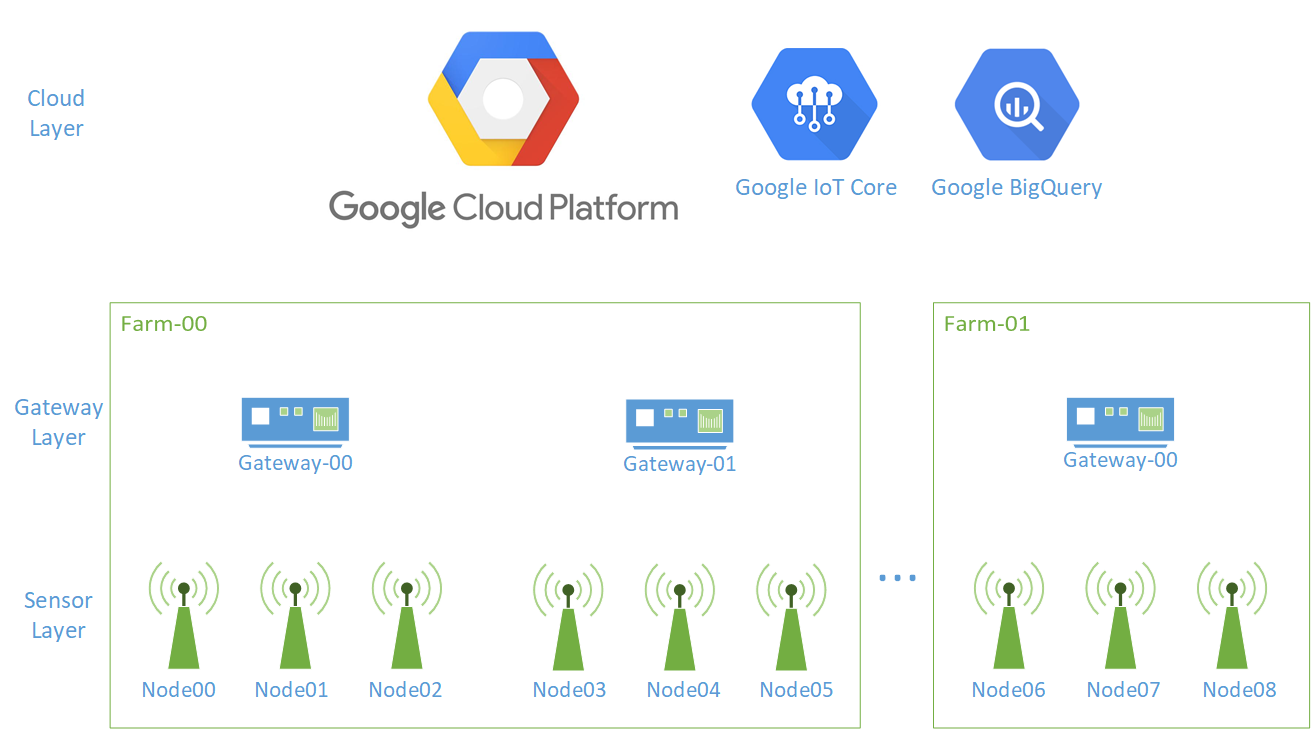
\includegraphics[width=\textwidth]{layers.png}
  \caption{Proposed 3-layer architecture}
  \label{fig:layers}
\end{figure}

\subsection{Sensor Layer}
  The sensor layer is comprised of the actual sensing hardware. Each device or node currently comprises of just 3 modules: an IoT capable micro-controller(NodeMCU ESP8266, see Figure~\ref{fig:nodemcu}), the environmental sensors (Soil Moisture and Temperature), and a 3.2v battery (LiFePo4). The functionally modular design allows for easy upgradability and repair. The node design schematics are given in Figure~\ref{fig:node}. Please note that the D0 pin (GPIO 16) needs to be connected to the RST pin of the ESP8266 to enable deep sleep, this needs to be disconnected to allow flashing of new firmware.

  \begin{figure}[!h]
    \centering
    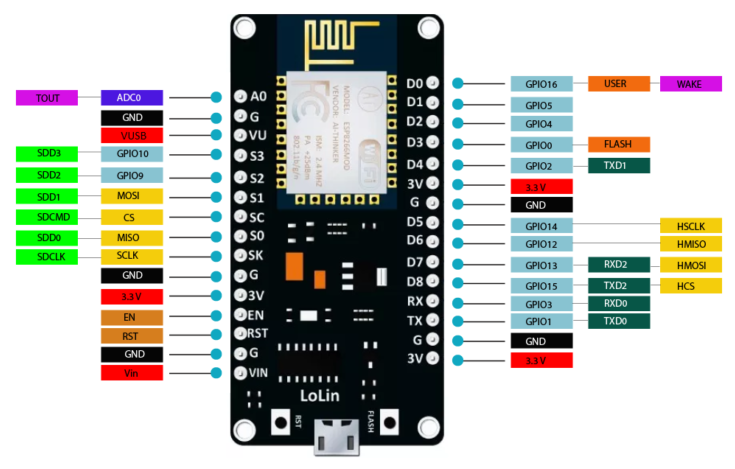
\includegraphics[width=0.9\textwidth]{nodemcu_pinout.png}
    \caption{NodeMCU ESP8266}
    \label{fig:nodemcu}
  \end{figure}
  
  \begin{figure}[!h]
    \centering
    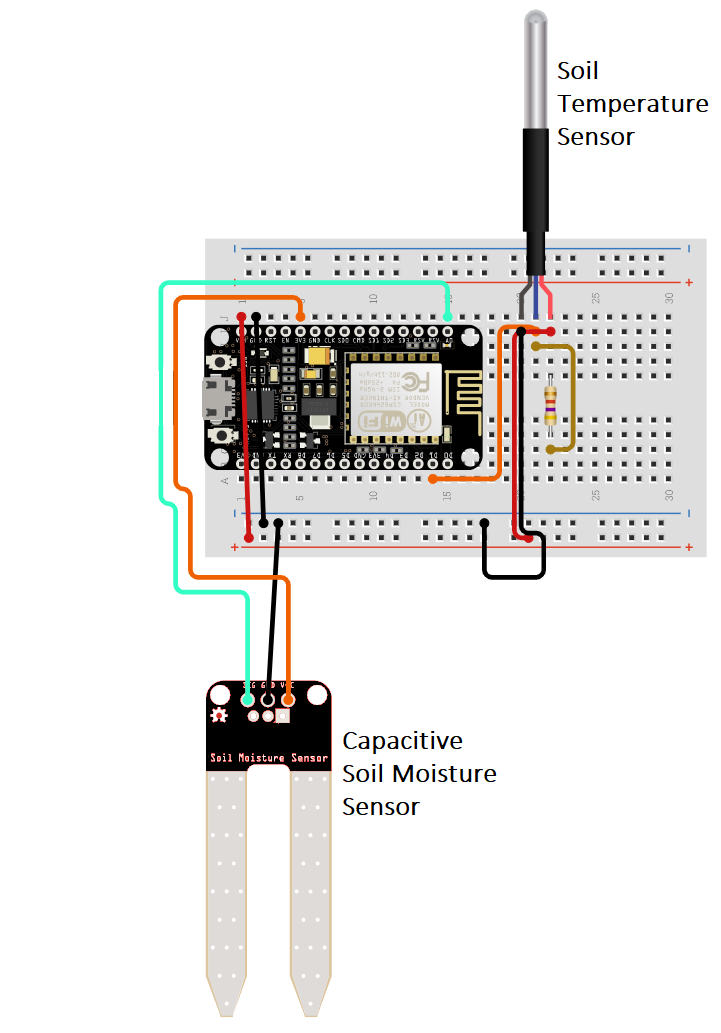
\includegraphics[width=0.7\textwidth]{node.png}
    \caption{Node Design Schematics}
    \label{fig:node}
  \end{figure}

  The ESP8266 microcontroller is a low-cost, low-power microcontroller with inbuilt WiFi capability and multiple GPIOs for communication purposes (Refer to Table~\ref{table:nodespecs}). The micro-controller is responsible for collecting the data from the sensors and sending it to the gateway through the mesh. The micro-controller is powered by a 3.3v power source and uses 80-90mA during load and 20\si{\micro\ampere} during deep sleep. Using a 1-3 hour duty cycle, the power consumption of the micro-controller can be reduced to less than 1mA per hour. Using a 3000mah battery, this can last anywhere from 150-215 days depending on external factors.
  
  \begin{table}[!h]
    \centering
    \begin{tabular}{ p{5cm} p{5cm}}
      \hline
      \textbf{Parameters} & \textbf{Specification}\\
      \hline
      Processor & TenSilica L106 80MHz 32bit\\
      SRAM & 160 kbytes\\
      Flash Storage & SPI Flash, up to 16 MBytes\\
      GPIO pins & 17\\
      ADC pins & 1 pin, 10 bit\\
      WiFi & 2.4GHz, 802.11 b/g/n\\
      Operating Voltage & 3-3.6 Volts\\
      \hline
    \end{tabular}
    \caption{ESP8266 (Sensor Node) Specifications} 
    \label{table:nodespecs}
  \end{table}

  \FloatBarrier
  \begin{table}[!h]
    \centering
    \begin{tabular}{ p{5cm} p{5cm}}
      \hline
      \textbf{Sensor} & \textbf{Model}\\
      \hline
      Soil Temperature & DS18B20\\
      Soil Moisture (Capacitive) & RKI-3225\\
      \hline
    \end{tabular}
    \caption{Used Sensor Models} 
    \label{table:sensors}
  \end{table}

\subsection{Gateway Layer}

  The gateway layer comprises aggregating devices that connect to WSN networks, collect the data, authenticate the devices, and then relay the data to the cloud. During each duty cycle, the gateway will wake up and perform the following:
  \begin{enumerate}
    \item Connect to the WSN using wifi;
    \item Authenticate active sensor nodes using a JSON Web Token (JWT);
    \item Collect sensor reading and calculate any derived measurements;
    \item Relay to Cloud MQTT broker and the BigQuery database for archival storage with proper timestamps; and
    \item Receive any configuration updates and relay them to the respective node in the WSN.
  \end{enumerate}
  The gateway is implemented using Raspberry Pi 4 (4GB) micro-controller (see Figure~\ref{fig:rpi}). Being equipped with a 1.5GHz quad-core CPU and 4 GB RAM, it is more than capable enough to handle multiple data streams and adds to the scalability of the design. These devices provide sufficient edge processing, removing any requirement for cloud-based processing power. The inbuilt WiFi(2.4 GHz and 5.0 GHz), Bluetooth 5.0, and BLE modules can be used for connecting to both Wifi and BLE based WSNs. A 4G USB dongle is used to provide internet connectivity in remote areas, but an ethernet interface can also be used for the same.

  \begin{figure}[!h]
    \centering
    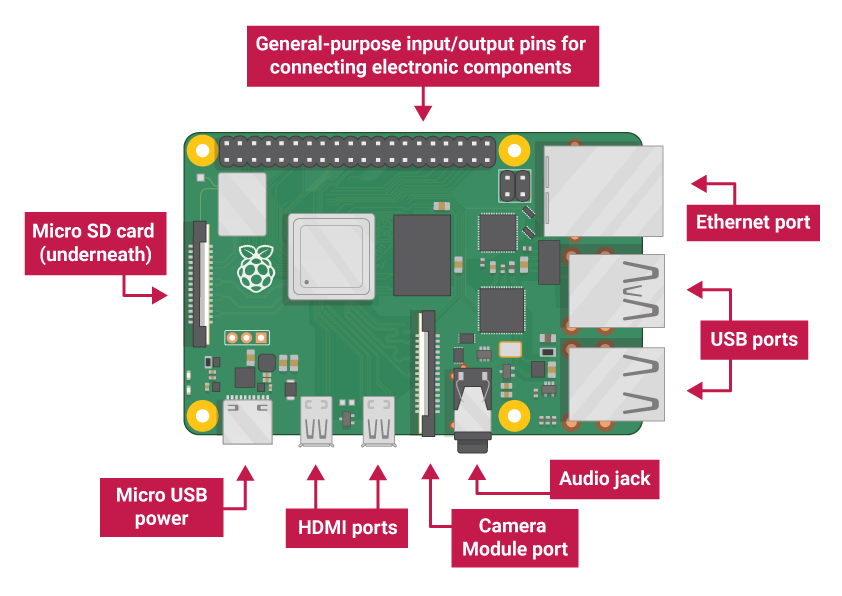
\includegraphics[width=\textwidth]{pi-labelled-names.png}
    \caption{Raspberry Pi 4}
    \label{fig:rpi}
  \end{figure}

  \FloatBarrier
\subsection{Cloud Layer}
  The cloud layer is responsible for data ingestion, device management through the gateway, and providing archival storage and data analytics. The cloud architecture is described in Figure~\ref{fig:cloud}.


  \begin{figure}[!h]
    \centering
    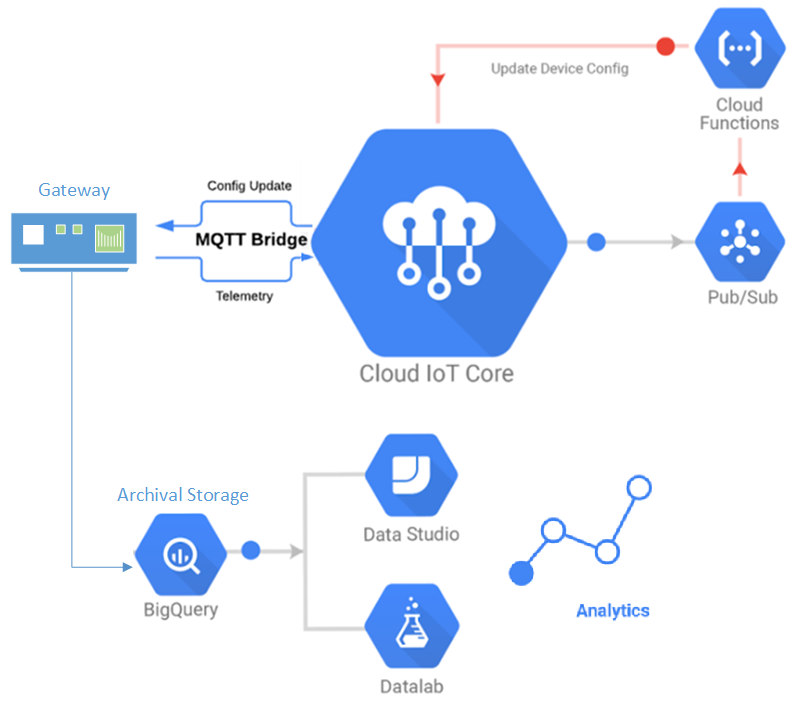
\includegraphics[width=0.9\textwidth]{cloud.png}
    \caption{GCP Cloud Architecture}
    \label{fig:cloud}
  \end{figure}  

  The Google Cloud Platform (GCP) is used for the same as Google Cloud IoT core platform has the functionality to support data ingestion from a large number of globally distributed devices. The platform also has integrated services that manage authentication and device management. Google BigQuery is used for archival storage and data analytics as it supports direct streams of data and has high throughput \cite{iotCore,ref1.13}. 
  
  A direct connection between an ESP8266-based node and Google Cloud IoT Core is possible but since many inexpensive boards lack the features required to make a secure connection, the WSN is kept isolated. The gateway layer handles the authentication process for the nodes through JSON Web Token (JWT) authentication. Each node must be authenticated via the gateway it is bound to before it can send any telemetry data.


\chapter{Solution Stack}
\section{Hardware Stack}

The two main factors that decided the hardware stack are cost and functionality. The node needs to be as inexpensive as possible as to keep the costs down when scaling, and the gateway needs to be powerful enough to allow easy scalability and upgradability.

The 2 microcontrollers that are a great fit to serve as the brain of the node, ESP8266 and ESP32. Both are perfectly suited and the software stack is compatible with both of them. To keep the development costs down, the ESP8266 was used.
The complete bill of materials is given in Table~\ref{table:billofmat}.

\renewcommand{\arraystretch}{1.2}
\begin{table}[h!]
\begin{tabular}{ p{2.3cm} p{6cm} p{1.3cm} p{1.3cm} }
    
    \hline
    \textbf{Device} & \textbf{Components} & \multicolumn{2}{l}{\textbf{Cost}}\\
    \hline
    9 x Nodes & & & \rupee~1,050
    \\
    & ESP8266 &\rupee~364 &
    \\
    & Soil Moisture Sensor&\rupee~177 &
    \\
    & DS18B20 Soil Temperature Sensor&\rupee~110 &
    \\
    & 3000mah LiFePo4 Battery&\rupee~299 &
    \\
    & Housing&\rupee~100 &
    \\\hline
    1 x Gateway & & & \rupee~5,272
    \\
    & Raspberry Pi 4 (4GB)&\rupee~3,994 &
    \\
    & 16GB Storage&\rupee~279 &
    \\
    & 4G Dongle&\rupee~999  &
    \\\hline
    Total: & & & \rupee~14,722 
    \\\hline

\end{tabular}
\caption{Bill of Materials}
\label{table:billofmat}
\end{table}



\section{Software Stack}

\subsection{Node}
    The ESP8266 node is programmed using PlatformIO~\cite{platformio}, an open-source, cross-platform IDE. This allows for fast debugging, code execution, and testing on any platform that can run python. The code is written in C++ (refer to Appendix 8.1).

    \noindent
    The mesh is built and configured using painlessMesh~\cite{painlessMesh} module, an open-source library that takes care of the particulars of creating a simple ad-hoc mesh network which required no central controller. It is compatible with both the ESP8266 and the ESP32. Each node created a wifi network with the same SSID but different BSSID. After the mesh is initialized and configured, only one SSID is publicly visible, reducing any network clutter.

    \noindent
    The main loop logic is defined as follows:
    \begin{enumerate}
        \item Initialize the mesh and wait for the gateway to connect (until max wait time);
        \item When connected, request for authentication, and sense the parameters;
        \item When authenticated, send the payload with the available parameters;
        \item Receive any configuration updates, or commands from the gateway and perform the necessary actions; and
        \item Go to deep sleep until the next wakeup cycle.
    \end{enumerate}

\subsection{Gateway}
    The gateway powered by the Raspberry Pi 4 hardware is programmed in python, allowing for cross-platform compatibility and support. The python script works alongside a modified version painlessMeshBoost library~\cite{painlessMeshBoost} which creates a bridge between the WSN mesh and the gateway.

    \noindent
    The setup instructions are as simple as running the python script with the appropriate arguments. The main loop logic is defined as follows:
    \begin{enumerate}
        \item Actively looks for the WSN and connect when available;
        \item When connected, using the painlessMeshBoost bridge receive the telemetry data from the Sensor nodes and act accordingly;
        \item Relay the telemetry data with appropriate timestamps to Google Cloud IoT Core, and BigQuery database for archival storage;
        \item Relay any configuration updates and commands to the specific nodes using the bridge; and
        \item Sleep until the next wakeup cycle.
    \end{enumerate}

\chapter{Full Deployment Process}

The link for the full code base is: \url{https://github.com/Raghav-intrigue/dfpl-project001}

\noindent
To download the full solution:

\begin{lstlisting}[tabsize=2,basicstyle=\footnotesize,language=bash,breaklines=true]
git clone --recurse-submodules \
	https://github.com/Raghav-intrigue/dfpl-project001
cd dfpl-project001
\end{lstlisting}

\noindent
Then, the deployment from scratch requires:

\subsection{Initial cloud setup}

   This will be done only once in the projects lifetime.
   \noindent
   Follow the instructions in \href{https://github.com/Raghav-intrigue/dfpl-project001/blob/master/documentation/cloud.md}{Cloud setup from scratch}

\subsection{Device setup and registration}

    Each device (node and gateway) has a unique ID, this needs to be registered on the cloud. This ID can be any arbitrary string (ensure consistency in the naming schema for convenience).
    \noindent
    This will be done once for each device in it's lifetime.
    
    \begin{enumerate}
    \item Setup Cloud (open \href{https://github.com/Raghav-intrigue/dfpl-project001/blob/master/documentation/cloud.md}{Cloud Setup}):
	    \begin{itemize}
	    \item Register Gateway (note down the gatewayID)
	    \item Register Nodes and Bind the nodes to the gateway (note the nodeIDs)
	    \end{itemize}
    \item Flash each node with the registered NodeIDs. See \href{https://github.com/Raghav-intrigue/dfpl-project001-node}{Node Setup}
    \item Setup Gateway (software installation). See section \href{https://github.com/Raghav-intrigue/dfpl-project001-gateway}{Gateway Setup}
    \end{enumerate}

\subsection{Field Deployment}
    \begin{enumerate}
    \item Turn on the gateway (Raspberry Pi)
	    \begin{itemize}
	    \item Connect the given USB C power adapter  to the raspberry pi.
	    \item Connect the given 4G dongle to raspberry pi via usb
	    \item Turn on the raspberry pi
	    \end{itemize}
    \item Place the nodes in the field
    \item Turn them on
    \end{enumerate}

\chapter{Next Steps}
The platform developed supports and is designed for various decision driven applications, which would include actuators and valves for controlling the amount of farm inputs. In the process of making the architecture industry ready, the following steps are needed:

\begin{itemize}
\item Designing a front end for platform management and deployment;
\item Designing industry-ready sensors for robust hardware and more reliable measurement;
\item Improving the mesh architecture for more stability; and
\item Adding field imagery and drone footage as sensory input.
\end{itemize}


\chapter{Code:}
\section{Code for Sensor Node}

\lstinputlisting[tabsize=2,basicstyle=\footnotesize,language=C++,breaklines=true]{content/code/node.cpp}

\section{Code for the gateway}
\lstinputlisting[tabsize=2,basicstyle=\footnotesize,language=Python,breaklines=true]{content/code/gateway.py}


\newpage
\addcontentsline{toc}{chapter}{References}
\printbibliography



\end{document}
